\documentclass[twoside,a4paper,12pt]{article}
\usepackage[applemac]{inputenc}
\usepackage{wrapfig}
\usepackage{graphicx}
\usepackage{graphics}
%\usepackage{subfig}
%\usepackage{inputenc}
\usepackage{amsmath}
\usepackage{amsfonts}
\usepackage{amssymb}
\usepackage[singlelinecheck=false]{caption}
\usepackage{array}
\usepackage{multirow}
\usepackage{setspace}
\usepackage{hyperref}
\usepackage{verbatim}
\usepackage[clearempty]{titlesec}
\usepackage{epstopdf}
\usepackage{lineno}
\usepackage{textcomp}
\usepackage{nicefrac}
\usepackage{xspace}
\usepackage{todonotes}
%\usepackage{autoref}
\usepackage[small, bf, hang, raggedright]{subfigure}

\usepackage[english]{babel} 

\onehalfspacing
\usepackage[left=2.9cm,right=2.9cm,top=3cm,bottom=4.5cm]{geometry}
\newcommand\leerseite{\newpage\thispagestyle{empty}\hspace{1cm}\newpage}

\newcommand{\subfigureautorefname}{\figurename}

\newcommand\piminus{\(\mathrm{\pi^-}\)}
\newcommand\muminus{\(\mathrm{\mu^-}\)}
\newcommand\eminus{\(\mathrm{e^-}\)}
\newcommand\eplus{\(\mathrm{e^+}\)}
\newcommand\geant{\textsc{Geant\,4}\xspace}

\begin{document}\selectlanguage{english}




\section*{Answers to Jerry's comments from 26.04.2016}
Dear Jerry,

I have tried to answer your questions below. I guess having a phone call will make things easier. However this phone call would need to happen very soon (as in today or possibly tomorrow). So if you have a time slot that fits you please tell me and we can try to arrange something. How about around 9AM your time today (assuming you are at NIU at the moment)?


\begin{quote}\texttt{With respect to plot 10b, I?d like to get a sense of how events with different characteristics move around, could you please cut the distribution on those events for which the energy found in the SECAL using the\\ 
1) standard reconstruction is <50\% \\
2) standard reconstruction is >50\%  \\
3) software compensating reconstruction is <50\% \\
4) software compensating reconstruction is >50\% \\
I don't see how this is circular argument at all since the em fraction is only part of the overall energy.}\end{quote}
Ok, I think I misunderstood your previous question, but just to make sure: The fraction of shower energy in electromagnetic sub-showers is a different quantity than the fraction of energy reconstructed in the ScECAL (with a significant correlation of course).

I have added the requested plots (for 32\,GeV data runs) below (\autoref{fig:jerry1} to \ref{fig:jerry4}). Events with high energy content in the ScECAL will have a higher EM-shower fraction, as hadronic showers can only be contained in the ScECAL when most of their energy goes into $\pi^0$ and thus EM sub-showers. There is practically no difference between the spectra selected on standard reconstruction AHCAL energy fraction and software compensation energy reconstruction. 

The stronger slope in the reconstructed energy correlation for low AHCAL energy fraction events observed around 40\,GeV standard reconstruction is due to the higher granularity and denser EM sub-showers in the ScECAL (the moliere radius of the ScECAL is around 1\,cm, while the moliere radius in the AHCAL is around 3\,cm), which makes software compensation more efficient. This effect is amplified by the slightly biased selection of showers with high EM fraction as explained above.  

The mean reconstructed energy fraction for 32\,GeV events is around 25\% energy in the ScECAL and around 75\% energy in the AHCAL, with wide distributions in both values due to the fluctuations in hadronic shower developments. For the same reason, the selection of AHCAL energy fraction $>50\%$ yields around 75\% of all events, while the selection on AHCAL energy fraction $<50\%$ yields only around 25\% of the events.

In addition to the plots you asked for, I plotted the correlation of reconstructed energy in the ScECAL in standard and SC reconstruction (\autoref{fig:jerry0}, from 32\,GeV \piminus data). For events with a large fraction of reconstructed energy in the ScECAL, software compensation tends to suppress the ScECAL energy fraction compared to the standard reconstruction due to the higher electromagnetic shower fraction in such events. 

I hope this helps.


\begin{figure}[hbt]
\begin{center}
\includegraphics[width=0.8\textwidth]{erec_ecal_standard_sc_jerry}
\caption{Correlation of reconstructed energy in the ScECAL in standard reconstruction vs. software compensation reconstruction. The dashed red line indicates the 1:1 correlation function. 32\,GeV \piminus (data).}
\label{fig:jerry0}
\end{center}
\end{figure}

\clearpage
\begin{figure}[t]
\begin{center}
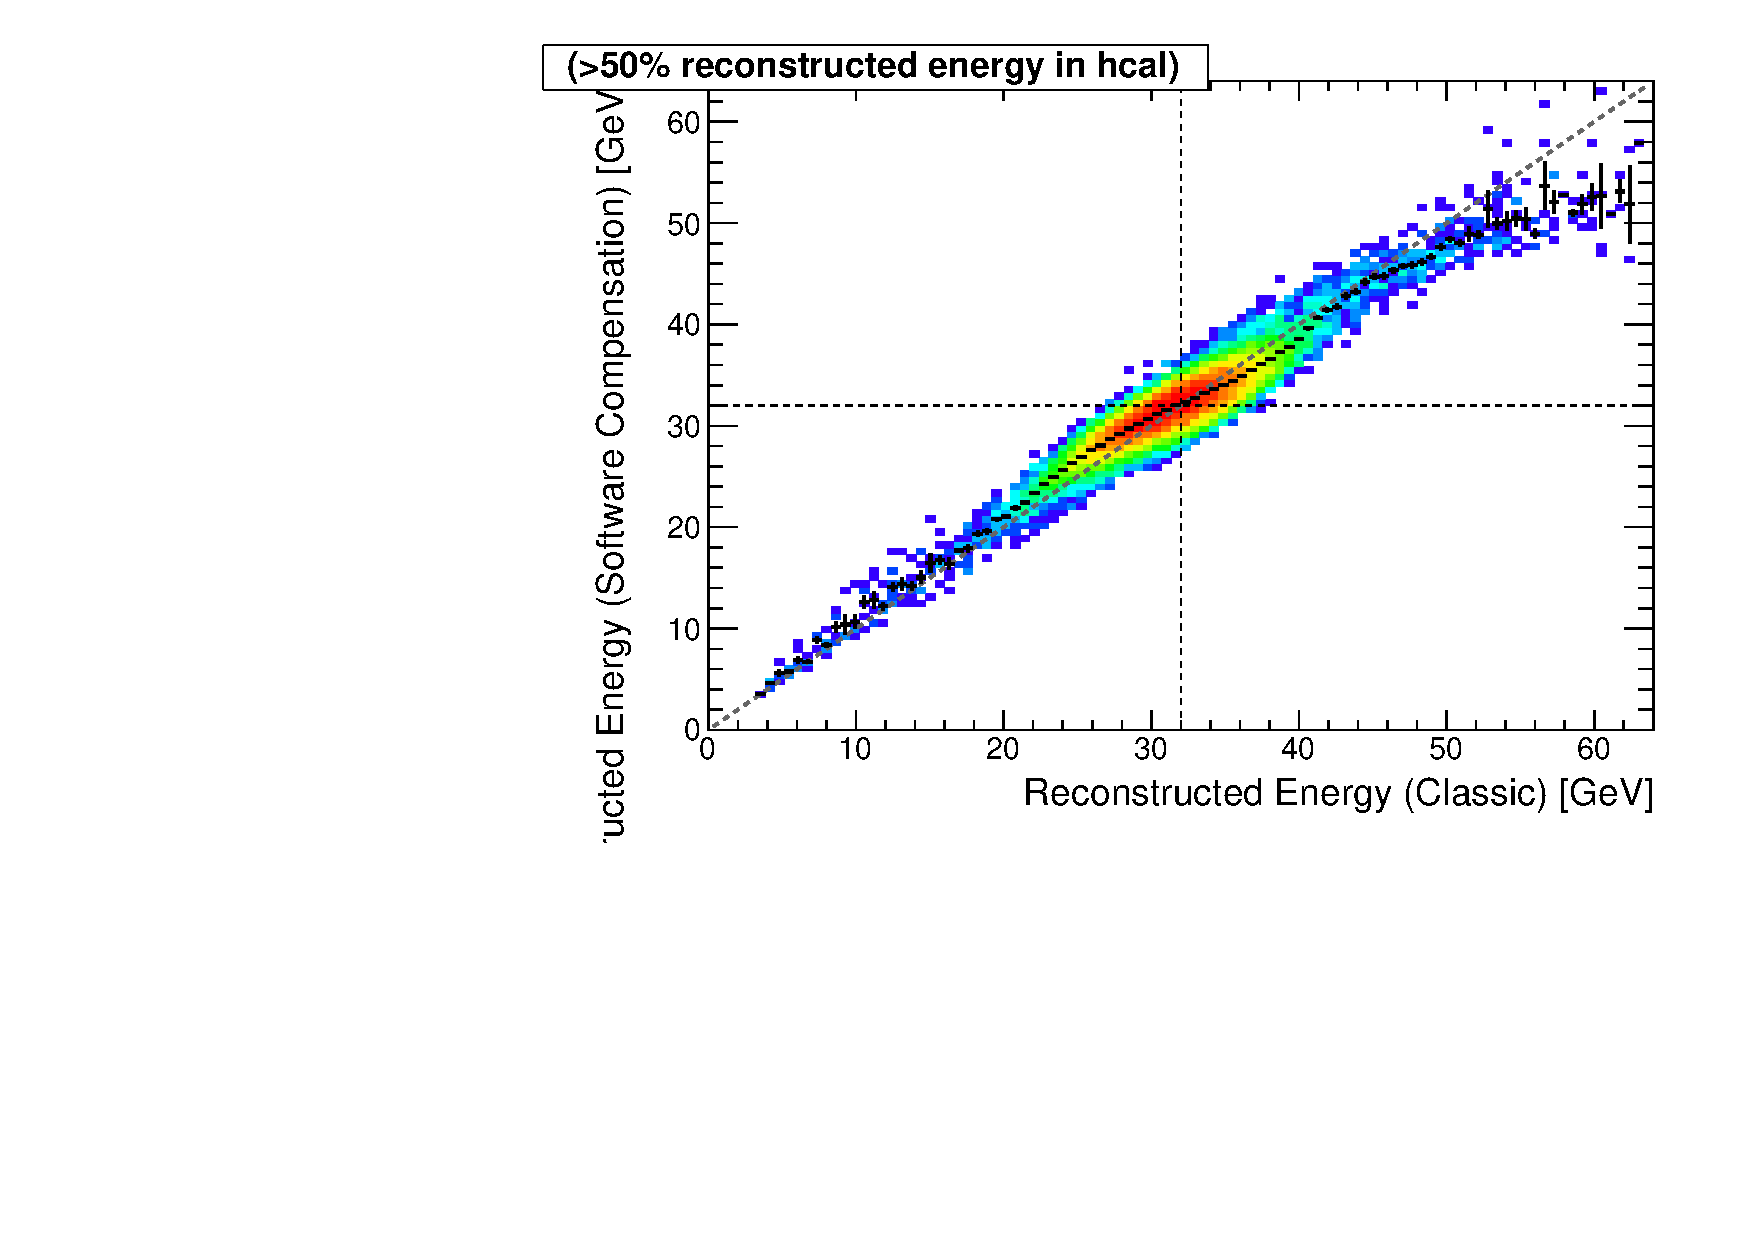
\includegraphics[width=0.8\textwidth,page=1]{ERec_corr_jerry_560474_data}
\caption{Correlation standard vs. software compensation reconstructed energy for event with $> 50\%$ of the standard reconstruction shower energy deposited in the AHCAL. 32\,GeV \piminus.}
\label{fig:jerry1}
\end{center}
\end{figure}
\begin{figure}[b]
\begin{center}
\includegraphics[width=0.8\textwidth,page=2]{ERec_corr_jerry_560474_data}
\caption{Correlation standard vs. software compensation reconstructed energy for event with $< 50\%$ of the standard reconstruction shower energy deposited in the AHCAL. 32\,GeV \piminus.}
\label{fig:jerry2}
\end{center}
\end{figure}
\begin{figure}[t]
\begin{center}
\includegraphics[width=0.8\textwidth,page=3]{ERec_corr_jerry_560474_data}
\caption{Correlation standard vs. software compensation reconstructed energy for event with $> 50\%$ of the SC reconstruction shower energy deposited in the AHCAL. 32\,GeV \piminus.}
\label{fig:jerry3}
\end{center}
\end{figure}
\begin{figure}[b]
\begin{center}
\includegraphics[width=0.8\textwidth,page=4]{ERec_corr_jerry_560474_data}
\caption{Correlation standard vs. software compensation reconstructed energy for event with $< 50\%$ of the SC reconstruction shower energy deposited in the AHCAL. 32\,GeV \piminus.}
\label{fig:jerry4}
\end{center}
\end{figure}

\clearpage
\begin{quote}\texttt{
1) Doe the sloped lines mean that the actual weight changes with the number of hits?}\end{quote}
No. The actual weight changes with 1/$e_\text{hit}$, cancelling out the hit energy and thus counting number of hits in this hit energy bin. I try to explain once more below.

\begin{quote}\texttt{2) How does one use the upper axis in Figures 9c and 9d labeled MIP?}\end{quote}
You use it to directly look up the appropriate weighting factor for a hit with a given hit energy.

Assume we want to do software compensation energy reconstruction of a given event with, for sake of simplicity, depositions only in the AHCAL. Let's assume we already ran the classic reconstruction on this event, from which we got an estimate of the shower energy E\_est = 4GeV.

To do the software compensation reconstruction, for each hit in the shower, we look up the appropriate software compensation weight from Figure 9(d) (The weights for an estimated shower energy of 4GeV are given in blue lines as examples). We then multiply the hit energy of the hit with the weight obtained from the lookup, and add up all these weighted hit energies to obtain our reconstructed shower energy. These weights are constant with hit energy for the bins 3--8 ($w_i = c_i$ for i = 3--8). In the first two bins, the bin weights are not constant, but are parametrised with a dependence on hit energy $e_\text{hit}$: $w_i = \frac{c_i}{e_\text{hit}}$ for i = 1--2. This is the slopes you see in the plot.

Assume in the given event we have an AHCAL hit with hit energy 10\,MIP. This will fall into AHCAL hit energy bin 4 and give a weight of around 0.75. So we add $10\,\text{MIP} \times 0.75 = 7.5\,\text{MIP}$ to our reconstructed energy sum. If the hit energy was only 8\,MIP or 9\,MIP, it would fall into the same hit energy bin and thus give the same SC weighting factor, but the contribution to the reconstructed energy would be proportional to the hit energy. This is ``normal'' summing up of hit energies.

Now assume the next AHCAL hit has an amplitude of 1\,MIP. We lookup the weight for a 1\,MIP hit and get something around 1.5, so we add $1\,\text{MIP} \times 1.5 \ = 1.5\,\text{MIP}$ to the reconstructed energy. However, a hit of 0.5\,MIP would \emph{not} give the same weight as a hit of 1\,MIP (even though they are both in the same hit energy bin!). Instead the weight looked up from Figure 9(d) for a hit of 0.5\,MIP is around 3, yielding a contribution to the reconstructed energy of $0.5\,\text{MIP} \times 3 \ = 1.5\,\text{MIP}$, exactly identical to the contribution of the 1\,MIP hit. All hits in the hit energy range of the first hit energy bin give the same contribution to the reconstructed shower energy, independent of their exact hit energy. This is the ``counting'' of hits in the first hit energy bin. 

% The simplified software compensation energy reconstruction (omitting the ScECAL and TCMT and the explicit weight dependence on the full shower energy) can be written as 
% \begin{align}
%   E_\text{rec}^\text{SC}=w_{\text{HCAL}} \cdot\left( \sum_{i}^{\text{hits}}\w_i\left(e_\text{hit}^i,E_\text{est.}\right)\cdot E^\text{HCAL}_i\right)
% \end{align}


\begin{quote}\texttt{
3) How does the upper axis help me help understand the plot? \\
4) Why not just have a different axis for Bins 1 and 2 instead of rescaling?}\end{quote}
Because this way of presenting hit energy dependent weights enables the direct comparison of practically any weighting scheme. For example, we can directly compare SDHCAL reconstruction weights (which only uses three counting bins overall) to our software compensation weights. If someone implements a different kind of hit energy based software compensation that does not rely on bins in the hit energy at all (by somehow parametrising the hit energy dependence of the SC weights), you could still show it in the same plot to compare. This would not be possible if one would base the whole plot on bins only. The comparison of different reconstruction schemes is not very relevant in this note, but the same way of presenting hit energy dependent weights is heavily used in the (soon to go into full collaboration review) CAN-49a. 

I believe this might get clearer if I switched the hit energy axis in these plots to the bottom part, so that it is clear that the actual x-axis is defined by the hit energy in MIPs, I will try to do that as soon as possible.

Cheers,
Oskar

\end{document}
